\label{sec:background}
\subsection{\acl{BDD}}
\label{subsec:bdd}
\acf{BDD} is a software development practice intricately woven into the framework of agile methodologies, that frames system design and development around end user expectations about the system and how it behaves~\cite{BDD_2006}. It positions itself as a dynamic response to prevalent challenges by prioritizing the user perspective and aligning closely with business needs. Based on the integration of concepts from both \ac{TDD} and \ac{DDD}, \ac{BDD} transcends traditional development paradigms~\cite{BDD_2006}.

\ac{BDD} stands out as a departure from the typical \ac{TDD} methodology, where the primary focus is on writing tests for isolated code units, with a predominant technical viewpoint, that restricts the determination of system behavior to developers and does not consider the system altogether. Instead, \ac{BDD} broadens its perspective, bridging the gap between technical and business aspects~\cite{Farooq2023bdd,Binamungu2020bdd}. It achieves this by incorporating viewpoints from both spheres, redirecting the evaluation from individual code segments to the holistic assessment of the application's behavior from the user's standpoint. This strategic change not only enhances communication, but also fosters collaboration between developers, testers, and business stakeholders, as evidenced by previous research~\cite{smart2023bdd,pereira2018behavior}.

Rooted in a user-centric philosophy, test cases are structured using a language that mirrors natural language, thus enabling non-technical stakeholders to define system behavior and overcoming the challenge of system design being solely within the realm of developers~\cite{BDD_2006}. This approach serves as a foundation for effective collaboration, creating a shared understanding among team members throughout the software development lifecycle.

\subsection{Gherkin}
\label{subsec:gherkin}

Gherkin is a \acf{DSL} prominently utilized in the domain of \ac{BDD}. It is used to create requirements and tests in a clear and human-readable format~\cite{noauthor_gherkin_nodate}. Gherkin's syntax follows a systematic Given-When-Then structure, interweaving natural language expressions, as demonstrated in \Cref{lst:withdrawcash}. Therefore, it focuses on the end-user's perspective and business requirements rather than the underlying technical implementation.

\begin{listing}[!ht]
\caption{Exemplary feature file with one scenario. Adapted from 
\href{https://cucumber.io/blog/bdd/getting-started-with-bdd-part-1/}{cucumber.io}~\cite{noauthor_getting_nodate}.}
\label{lst:withdrawcash}
\inputminted[linenos, xleftmargin=2em]{gherkin}{files/code/atm.feature}
\end{listing}

Gherkin employs a distinct set of keywords to delineate various aspects of test scenarios~\cite{noauthor_gherkin_nodate}. In particular, it utilizes the \texttt{feature} keyword to expound upon the primary functionality of the feature under examination, \texttt{Scenario} to specify individual use cases within the feature, \texttt{Given}-steps to establish initial context or preconditions, \texttt{When}-steps for denoting the event or action that triggers the scenario, and \texttt{Then}-steps for articulating anticipated outcomes for validation\footnote{It is imperative to acknowledge that this chapter does not exhaustively cover all Gherkin keywords, but rather focuses on those pertinent to our study~\cite{noauthor_gherkin_nodate}. A comprehensive list is available at \href{https://cucumber.io/docs/gherkin/reference/\#keywords}{https://cucumber.io/docs/gherkin/reference}}. Furthermore, the \texttt{And} keyword facilitates the chaining of multiple steps of the same type, ensuring a logically granular and encapsulated representation of test steps. 

This structural arrangement cultivates a shared understanding among stakeholders about the expected behavior of the system, thereby mitigating possible misunderstandings between shareholders and the development team.

\subsection{Cucumber}
\label{subsec:cucumber}
Cucumber\footnote{https://cucumber.io/} is open source software primarily utilized to perform \ac{BDD} tests. The Cucumber Open platform offers libraries for various programming languages, such as Java, JavaScript, Ruby, .NET, and others, providing all the essential functionality needed for parsing Gherkin files and execute tests up on them~\cite{noauthor_cucumber_nodate}. This is achieved by offering the functionality to map natural language descriptions of software requirements, found in Gherkin files, to specific test implementation steps. This comprehensive functionality facilitates the execution of Gherkin-based automated tests, effectively linking natural language descriptions to executable code~\cite{wynne2012cucumber}.

\begin{figure}
    \centering
    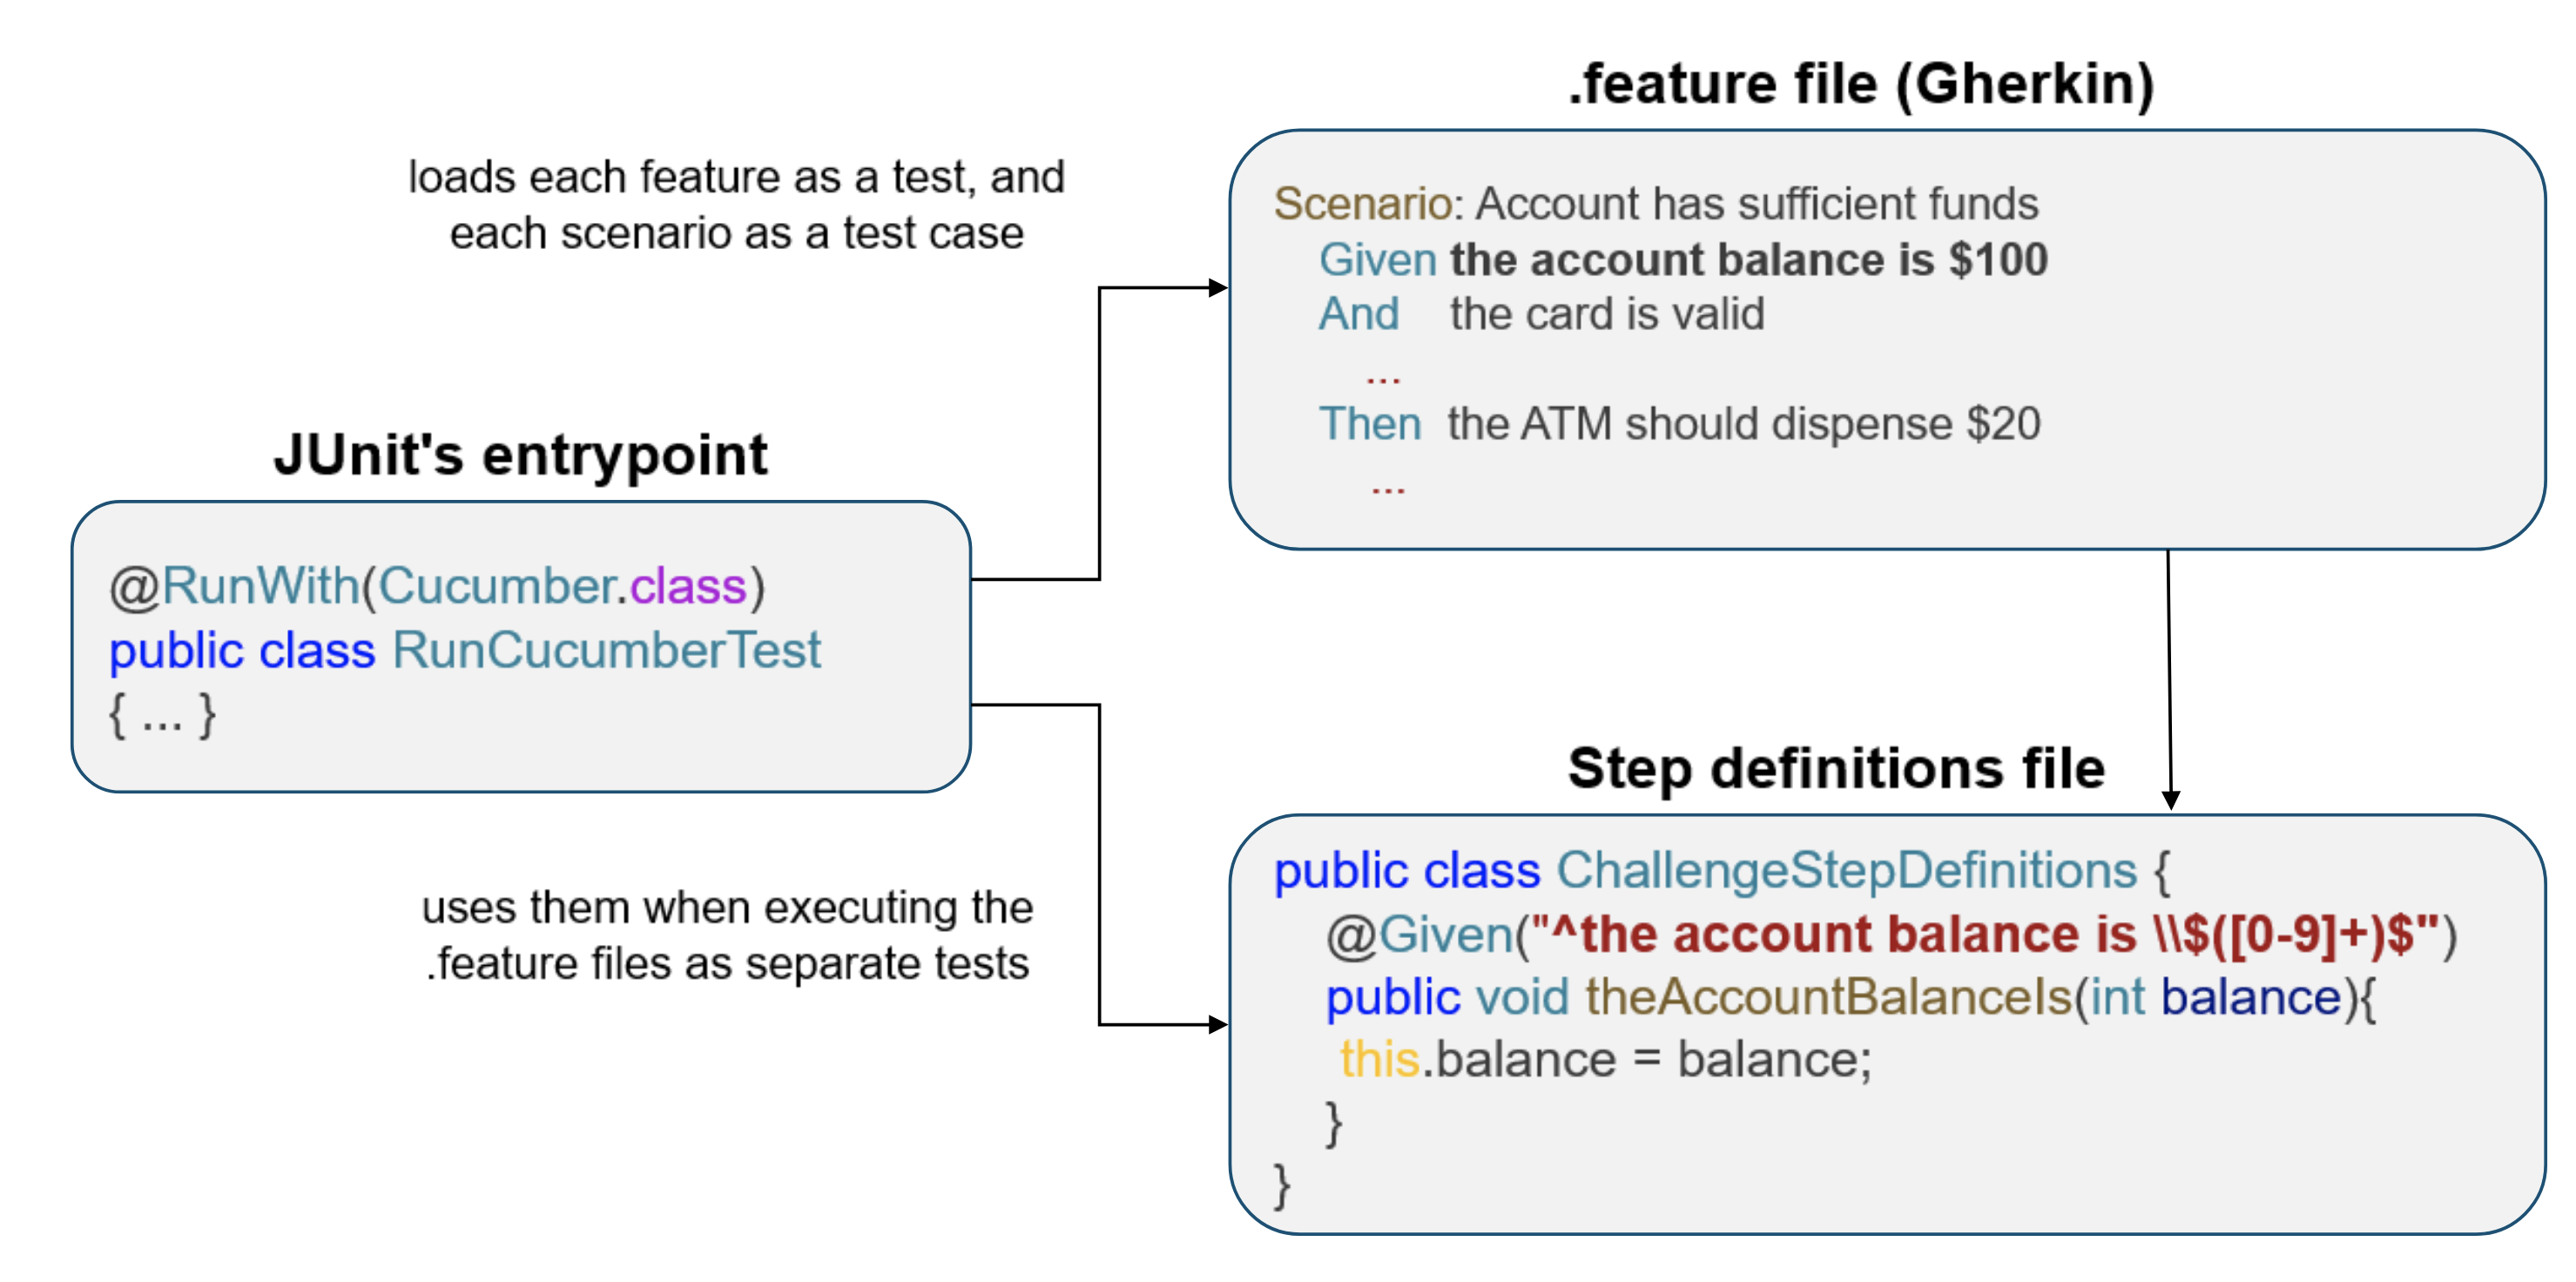
\includegraphics[width=\linewidth]{files/figures/cucumber_test_step_mapping.png}
    \caption{Illustration how Cucumber is used to link natural language clauses and their respective Java implementations. Adapted from thepracticaldeveloper.com~\cite{thepracticaldeveloperIntroductionMicroservice}}
    \label{fig:cucumber-mapping}
\end{figure}

Based on the scenario described in~\Cref{lst:withdrawcash}, the corresponding~\Cref{fig:cucumber-mapping} illustrates the connection between the specified natural language test steps and their concrete code representations. In the context of Java, developers use annotations to specify Java methods as implementations of steps in a Gherkin file. These annotations include a regex string that, when matched in a sentence, triggers the execution of the corresponding Java method. For instance, the \texttt{theAccountBalanceIs} function, annotated with \texttt{@Given}, is invoked when the regex matches a sentence, for example, ``the account balance is \$100`` in a ``GIVEN`` clause~\cite{noauthor_bdd_nodate}.

\subsection{Distributed Systems}
\label{subsec:dissys}
A distributed system is a network of independent computers, running on multiple servers or nodes, that interact and synchronize their activities through the exchange of information~\cite{tanenbaum2007distributed}. These systems consist of components that collaboratively work towards a shared objective, presenting advantages in terms of performance, scalability, and redundancy when compared to centralized systems. The shift from centralized architectures to distributed systems is driven by several inadequacies associated with non-distributed, centralized computing models, typified by a single monolithic server. Such centralized models have proven insufficient in addressing the increasing computational requirements and the need for enhanced system capabilities that could not be mitigated by vertically scaling a single system.

The distinctive feature of distributed systems lies in their avoidance of shared computing and memory resources, introducing complexities related to heterogeneity, scalability, and failure handling, among other challenges~\cite{coulouris2005distributed}. Non-distributed systems may struggle to effectively manage these challenges, leading to limitations in performance, scalability, and fault tolerance. Distributed systems, by distributing computational tasks across a network of interconnected computers, address these shortcomings~\cite{coulouris2005distributed}.

For instance, consider a scenario where a centralized system, operating on a single powerful server, reaches the maximum capacity of available hardware resources. Upgrading the hardware of that single machine (vertically scaling), may become impractical or cost-prohibitive. In such situations, distributed systems offer a viable solution. By distributing the workload across multiple interconnected nodes, these systems enable parallel processing, allowing for efficient utilization of available resources beyond the constraints of a single machine. 

However, this comes at the cost of complexity, as these clusters of individual computers need to be carefully coordinated and managed. Additionally, information must be transferred from one host to another, introducing non-determinism, particularly through the network, as a source of unpredictability. This introduces the potential for errors, such as when network packets are lost during the communication between nodes.

\subsection{\acl{RCE}}
\label{subsec:rce}
\acf{RCE}\footnote{https://rcenvironment.de/} is an open-source software that aids engineers, scientists, and other professionals in creating, managing, and executing complex calculation and simulation workflows~\cite{BODEN2021100759,rceDevGuide10x}. In RCE, a workflow consists of components with pre-defined inputs and outputs that are connected to each other. These components can be simulation tools, tools for data access, or user-defined scripts. The connections between the components determine the flow of data from one component to another~\cite{BODEN2021100759,rceDevGuide10x}. The software includes predefined components with common functionalities, such as an optimizer or a cluster component. Additionally, users can integrate their own tools. RCE instances can be connected with each other, and components can be executed locally or remotely on RCE instances, provided the component is configured to allow this~\cite{BODEN2021100759,rceDevGuide10x}. By using these building blocks, RCE enables the solution of use cases for complex distributed applications.

\subsection{Kubernetes}
\label{subsec:kubernetes}
\acf{K8S}\footnote{https://kubernetes.io/} is an open source container orchestration platform that has emerged as a foundational element in the development of modern native cloud applications. Originally developed by Google and presently overseen by the \ac{CNCF}, \ac{K8S} serves as a versatile and powerful solution to automate the deployment, scaling, and administration of containerized applications~\cite{burns2022kubernetes}. Its architectural design facilitates the abstraction of infrastructure intricacies, providing developers with a standardized environment for the efficient deployment and management of microservices~\cite{noauthor_production-grade_nodate}.


\subsection{Chaos Mesh}
\label{subsec:chaosmesh}
Chaos Mesh is an open source chaos engineering platform that facilitates systematic testing and identification of weaknesses in distributed systems~\cite{noauthor_chaos_nodate}. Developed by the Chaos Mesh community, it provides a versatile set of tools for inducing chaos experiments within \hyperref[subsec:kubernetes]{K8s} environments. These experiments aim to simulate real-world system failures and assess how well the system can withstand unexpected disruptions.

Chaos Mesh offers features such as fault injection, resource consumption testing, and network chaos, allowing users to replicate scenarios such as network delays, packet loss, and more. By orchestrating controlled chaos experiments, Chaos Mesh helps teams proactively discover and address potential vulnerabilities, leading to enhanced system resilience and reliability~\cite{noauthor_chaos_nodate}.

\subsection{WinDivert}
\label{subsec:windivert}
WinDivert\footnote{https://github.com/basil00/Divert} is a dynamic and versatile open-source library targeting Windows operating systems~\cite{noauthor_windivert:_nodate}. Developed by Basil Hussain, it provides a packet capture-and-divert framework that enables the interception, modification, and drop of network packets.

\begin{figure}
    \centering
    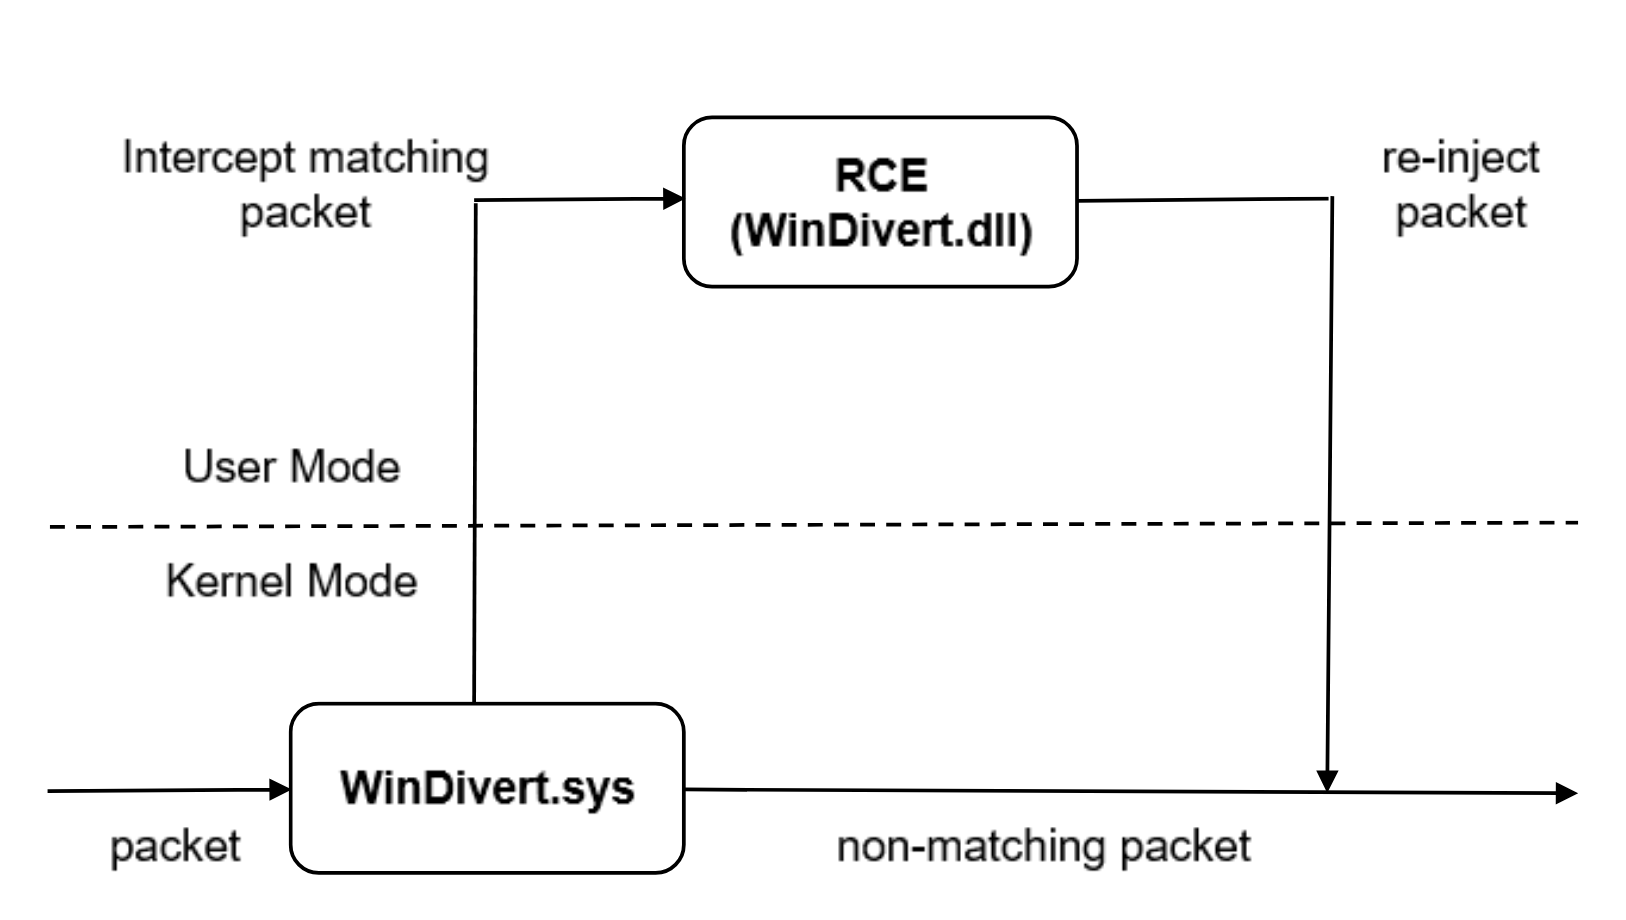
\includegraphics[width=\linewidth]{files/figures/WinDivert.png}
    \caption{WinDivert Architecture. Adapted from the WinDivert repository~\cite{noauthor_windivert:_nodate}.}
    \label{fig:WinDivert}
\end{figure}

As illustrated in~\Cref{fig:WinDivert}, WinDivert operates at the kernel level, but can be controlled from user mode, allowing user mode applications to exert fine-grained control over network traffic~\cite{noauthor_windivert:_nodate}. This capability facilitates the implementation of network-related functionalities, including firewall applications, intrusion detection systems, and network testing tools, directly within user-mode applications. With its Java bindings, WinDivert can be seamlessly integrated into Java applications, making it an attractive choice for scenarios where precise control over network traffic is essential~\cite{noauthor_windivert:_nodate}.